\documentclass[
	12pt,				% tamanho da fonte
	oneside,			% para impressão em recto e verso. Oposto a oneside
	a4paper,			% tamanho do papel. 
	english,			% idioma adicional para hifenização
	brazil,				% o último idioma é o principal do documento
	]{abntex2}

% ---
% Pacotes fundamentais 
% ---
\usepackage{lmodern}			% Usa a fonte Latin Modern
\usepackage[T1]{fontenc}		% Selecao de codigos de fonte.
\usepackage[utf8]{inputenc}		% Codificacao do documento (conversão automática dos acentos)
\usepackage{indentfirst}		% Indenta o primeiro parágrafo de cada seção.
\usepackage{color}				% Controle das cores
\usepackage{graphicx}			% Inclusão de gráficos
\usepackage{microtype} 			% para melhorias de justificação
\usepackage{multicol}
\usepackage{multirow}
\usepackage[brazilian,hyperpageref]{backref}	 % Paginas com as citações na bibl
\usepackage[alf]{abntex2cite}	% Citações padrão ABNT
\usepackage{listings}
\usepackage{float}

\lstset{
  showspaces=false,
  showtabs=false,
  breaklines=true,
  showstringspaces=false,
  breakatwhitespace=true,
  commentstyle=\color{green},
  keywordstyle=\color{blue},
  stringstyle=\color{red},
  basicstyle=\ttfamily
}

% --- 
% CONFIGURAÇÕES DE PACOTES
% --- 

% ---
% Configurações do pacote backref
% Usado sem a opção hyperpageref de backref
\renewcommand{\backrefpagesname}{Citado na(s) página(s):~}
% Texto padrão antes do número das páginas
\renewcommand{\backref}{}
% Define os textos da citação
\renewcommand*{\backrefalt}[4]{
	\ifcase #1 %
		Nenhuma citação no texto.%
	\or
		Citado na página #2.%
	\else
		Citado #1 vezes nas páginas #2.%
	\fi}%
% ---

% ---
% Informações de dados para CAPA e FOLHA DE ROSTO
% ---
\titulo{Prática 7: Batalha Naval em Rede}
\autor{Pedro Inácio Rodrigues Pontes}
\local{Belo Horizonte, Brasil}
\data{2025}
\instituicao{%
  Universidade Federal de Minas Gerais
  \par
  Colégio Técnico
  \par
  Curso Técnico em Desenvolvimento de Sistemas}

\definecolor{blue}{RGB}{41,5,195}

\makeatletter
\hypersetup{
     	%pagebackref=true,
		pdftitle={\@title}, 
		pdfauthor={\@author},
    	pdfsubject={\imprimirpreambulo},
		colorlinks=true,       		% false: boxed links; true: colored links
    	linkcolor=blue,          	% color of internal links
    	citecolor=blue,        		% color of links to bibliography
    	filecolor=magenta,      		% color of file links
		urlcolor=blue,
		bookmarksdepth=4
}
\makeatother

\renewcommand{\thesection}{\arabic{section}}
\setlength{\parindent}{1.3cm}
\setlength{\parskip}{0.2cm} 

\makeindex


\begin{document}

\selectlanguage{brazil}
\frenchspacing 

\imprimircapa

{
\ABNTEXchapterfont

\textual

% ----------------------------------------------------------
% Introdução (exemplo de capítulo sem numeração, mas presente no Sumário)
% ----------------------------------------------------------
\section{Introdução}

Objetivo: Desenvolver dois programas de Console Application em C# que se comuniquem via TCP para simular um jogo de Batalha Naval em um tabuleiro 10×10, com 10 navios de tamanho 1 posicionados pelo Servidor (Player 1) e ataques enviados pelo Cliente (Player 2).

\section{Desenvolvimento}

\subsection{Infraestrutura}

Como base para o jogo, foram criadas classes na pasta BatalhaNaval.Core:

\begin{itemize}
    \item Coordinate

    Representa as coordenadas. Pode receber uma tupla os inteiros linhas e coluna ou uma string no formato letra + número em seu construtor. Possui as variáveis \textit{Row}, \textit{Column} e \textit{Value} (tupla com as duas variávies anteriores. Possui o método \textit{MapValue} que converte a string dada no construtor para o valor suportado em \textit{Value}
    \item TableBase

    Classe abstrata que será herdada pelas classes que representam as mesas do player um e dois. Possui os métodos \textit{Initialilze}, \texit{Show} (mais seus complementares) e \textit{UpdateCell}
    \item IConsole

    Interface do Console com os métodos textit{Write}, textit{Read} e textit{ReadLine}. Feita como injeção de dependência para facilitar os testes unitários, que testei uso nesse exercício.
    \item IMessageStream

    Interface do NetworkStream. Feita para permitir injeção de dependência que vem a facilitar testes unitários. Possui os métodos \textit{Send}, \textit {Receive} e \textit{Close}
    \item SystemConsole

    Implementação do IConsole
    \item NetwrokMessageStream

    Implementação do NetworkStream
\end{itemize}

\subsection{Player1}
Representa a logística do  Player 1, o qual posiciona os navios no tabuleiro, de forma automática ou manual, além de ser o servidor TCP no qual o Player 2 irá entrar.

\begin{itemize}
    \item Menu

    Representa o menu inicial, no qual o player recebe as boas-vindas e pode escolher entre o posicionamento manual e automático. Possui os métodos \textit{Show}, \textit{ShowInitialMessage}, \textit{ProcessOption} e \textit{ReadOption}
    \item Ship

    Representa um navio no jogo. Tem as propriedades \textit{Coords} (do tipo Coordinate) e \textit{Sink} (bool). Possui o método \textit{IsHit}, o qual é autodescritivo e booleano.
    \item Server

    Cria o servidor TCP. Métodos \textit{Send}, \texit{Receive}, \textit{Close} e \textit{AcceptConnection} (utilizado para iniciar o servidor fora do ambiente de testes)
    \item Table

    Representa o tabuleiro do jogo. Tem métodos para criar a mesa com posições aleatórias ou manuais e receber o ataque do player2 e retornar a mensagem de feedback quanto ao acerto, erro ou vitória, além dos métodos complementares para que as funções funcionem corretamente.
    \item Program

    Implementa a solução. Mostra o menu, inicia o server e roda uma sequência de receber a mensagem do player2, processá-la e retornar o feedback a ele.
    \end{itemize}

\subsubsection{Demonstrações}
Implementação de Table (apenas os métodos públicos):

\begin{lstlisting}
public class Table : TableBase
{
    private const int MaxShips = 10;
    private readonly Random _rand;
    int _shipsNumber = 0;
    Ship[] _ships;

    public Table(IConsole console, Random? random = null) : base(console)
    {
        _rand = random ?? new Random();
        _ships = new Ship[MaxShips];
    }

    public void CreateTableWithRandomShipsPositions()
    {
        AddShipsRandomly();
        Show();
    }

    public void CreateTableWithManualShipPositions()
    {
        AddShipsManually();
        Show();
    }

    public string ReceiveAttack(string attack)
    {
        Coordinate attackCoordinates = new Coordinate(attack);
        foreach (var ship in _ships)
        {
            if (ship.IsHit(attackCoordinates))
            {
                _table[ship.Coords.Row, ship.Coords.Column] = 'X';
                Show();
                return IsGameWin() ? "WIN" : "HIT";
            }
        }
        _table[attackCoordinates.Row, attackCoordinates.Column] = 'O';
        Show();
        return "MISS";
    }

    public bool IsGameWin()
    {
        return _ships.Take(_shipsNumber).All(ship => ship.Sink);
    }
}
\end{lstlisting}

Implementação de Program

\begin{lstlisting}
var console = new SystemConsole();
var table = new Table(console);
var menu = new Menu(console, table);

menu.Show();

var server = new Server(15000);

while (!table.IsGameWin())
{
    var message = server.Receive();

    var attackStatus = table.ReceiveAttack(message);
    server.Send(attackStatus);
}
\end{lstlisting}

\subsection{Player2}

Implementa a dinâmica de ataque e estabelece conexão de cliente com o server do player1.

Seguem suas classes:
\begin{itemize}
    \item Client

    Estabelece a conexão cliente com o server player1.
    \item AttackTable

    Implementa a lógica de ataque e exibição do tabuleiro.
    \item Program

    Implementa a solução. Cria o cliente TCP e utiliza o método Play de AttackTable
\end{itemize}

\subsubsection{Demonstrações}

Implementação de AttackTable (apenas os métodos públicos):
\begin{lstlisting}
public class AttackTable : TableBase
{
    List<Coordinate> attackedCells = new();
    Client _client;
    string lastAttackStatus = "";

    public AttackTable(IConsole console, Client client) : base(console)
    {
        _client = client;
    }

    public void Play()
    {
        Show();
        while (lastAttackStatus != "WIN")
        {
            var coordinate = ReadAttackCoordinate();
            if (IsValidCoordinate(coordinate))
            {
                SendCoordinateToServer(coordinate);
                VerifyAttackStatus(coordinate);
            }
        }
    }
}
\end{lstlisting}

Implementação de Program
\begin{lstlisting}
IConsole console = new SystemConsole();
console.WriteLine("Bem vindo ao jogo Batalha Naval!");
Client client = new("127.0.0.1", 15000);
AttackTable table = new(console, client);
table.Play();
client.Close();
\end{lstlisting}

\section{Resultados}

\begin{figure}[H]
    \centering
    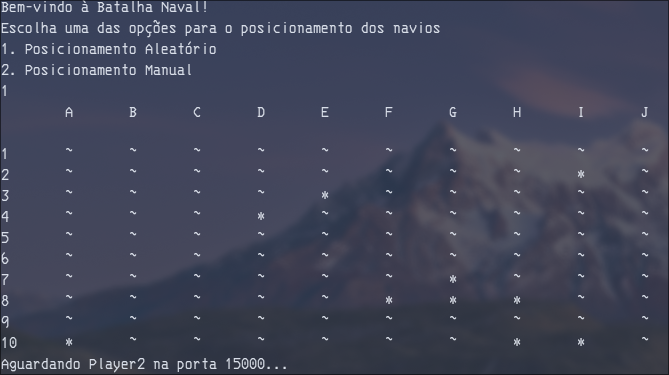
\includegraphics[width=1\textwidth]{imgs/player1-posicionamento-aleatorio.png}
    \caption{layer1-posicionamento-aleatorio.png}
    \label{fig:img1}
\end{figure}
\begin{figure}[H]
    \centering
    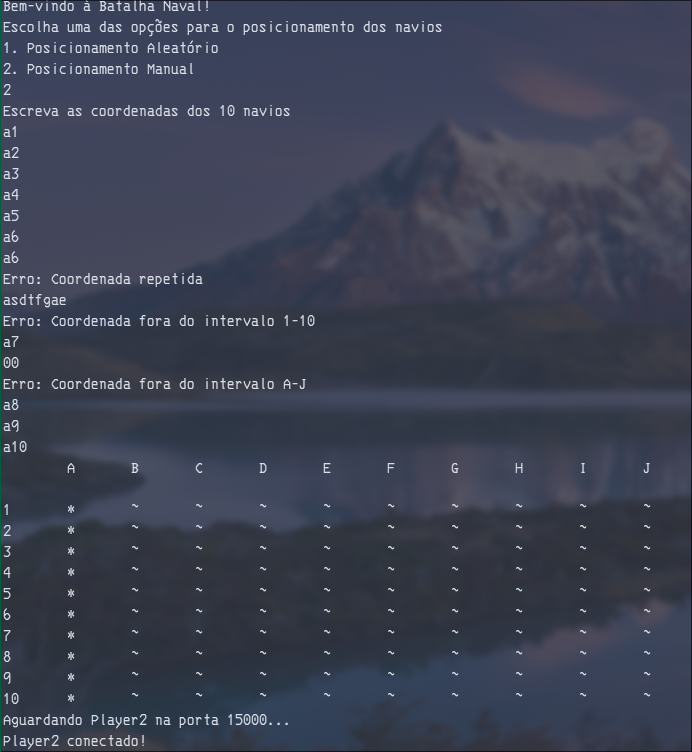
\includegraphics[width=1\textwidth]{imgs/player1-posicionamento-manual.png}
    \caption{player1-posicionamento-manual.png}
    \label{fig:img1}
\end{figure}
\begin{figure}[H]
    \centering
    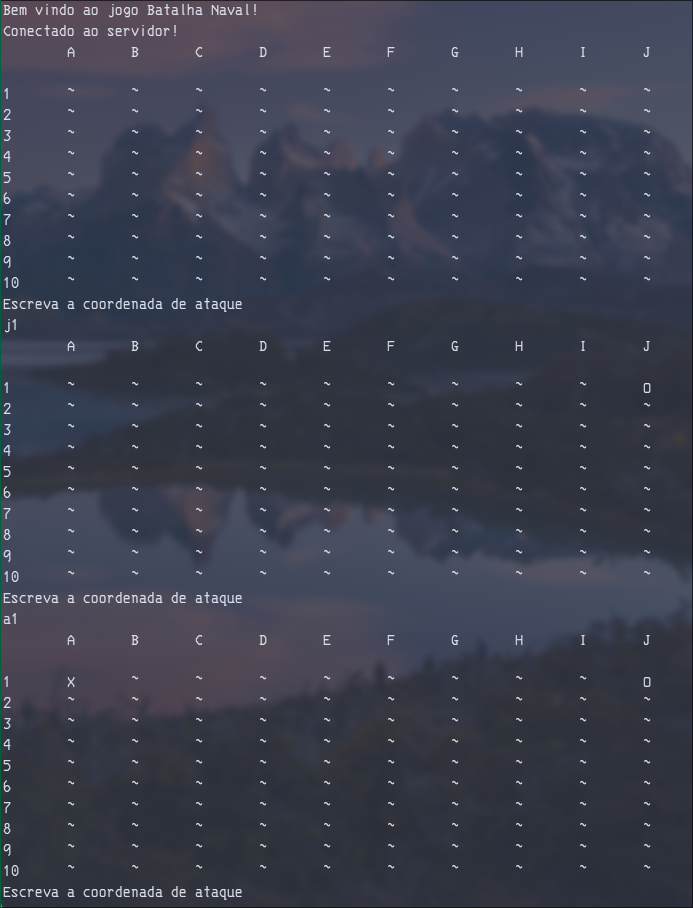
\includegraphics[width=1\textwidth]{imgs/player2-inicio-jogo}
    \caption{player2-inicio-jogo}
    \label{fig:img1}
\end{figure}
\begin{figure}[H]
    \centering
    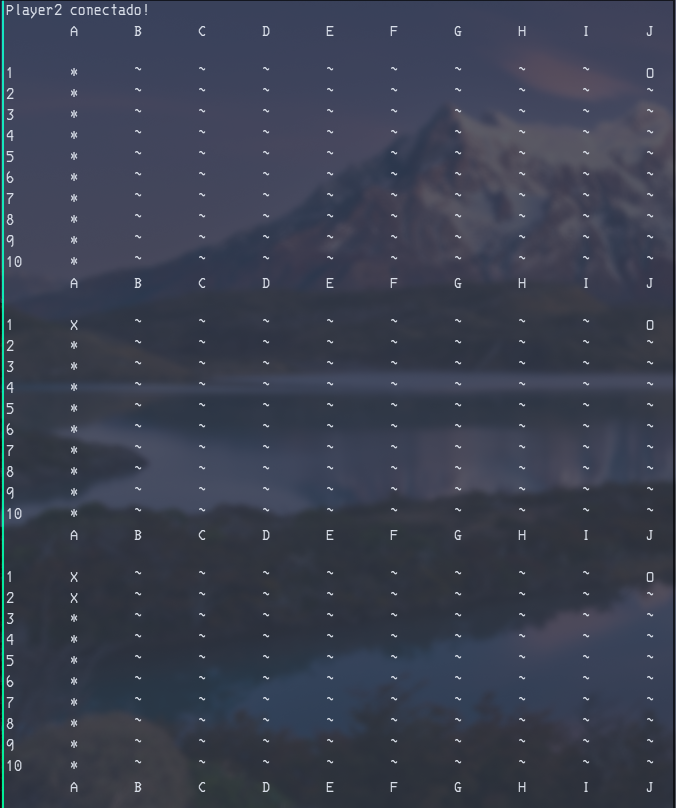
\includegraphics[width=1\textwidth]{imgs/player1-inicio-jogo}
    \caption{player1-inicio-jogo}
    \label{fig:img1}
\end{figure}
\begin{figure}[H]
    \centering
    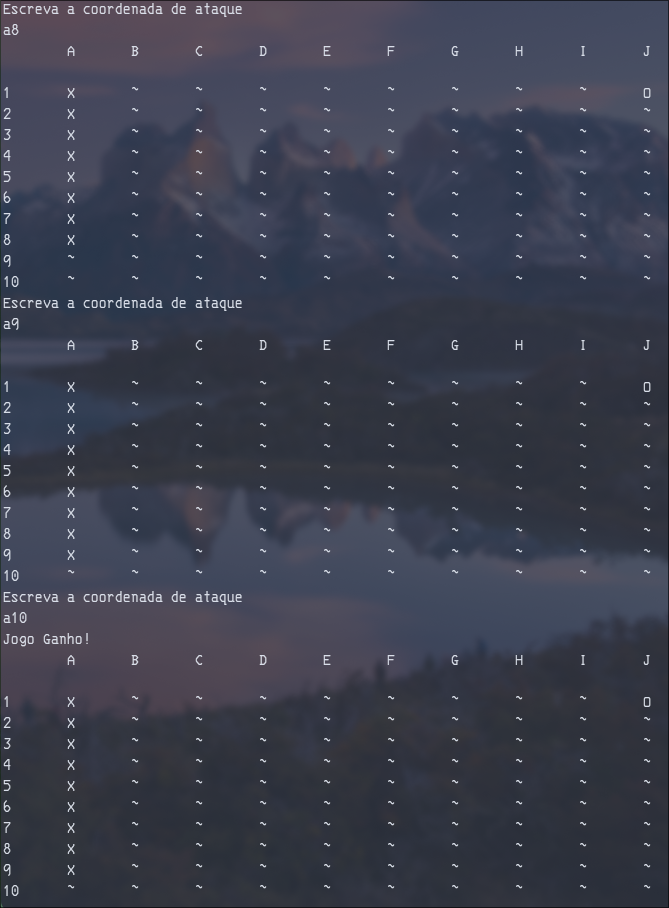
\includegraphics[width=1\textwidth]{imgs/player2-fim-jogo}
    \caption{player2-fim-jogo}
    \label{fig:img1}
\end{figure}
\begin{figure}[H]
    \centering
    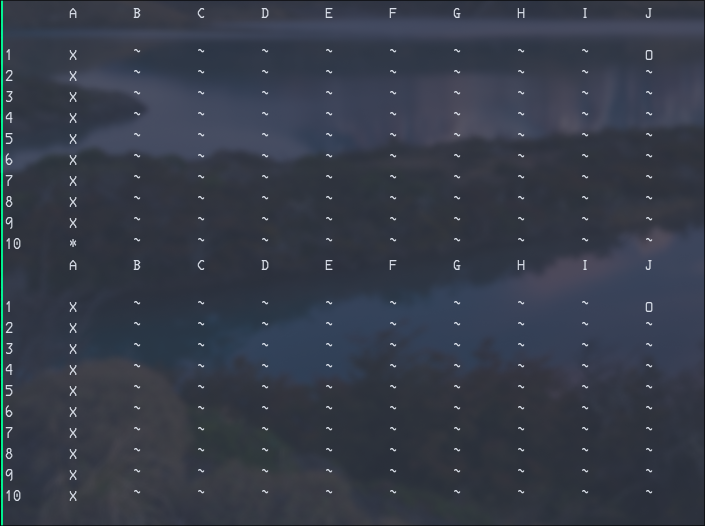
\includegraphics[width=1\textwidth]{imgs/player1-fim-jogo}
    \caption{player1-fim-jogo}
    \label{fig:img1}
\end{figure}

\section{Conclusão}

Todos os resultados foram alcançados. A implementação de testes unitários fez a criação da solução se estender por horas a mais do que deveria, pois estes forçam o código a estar bem feito. Tal coisa gerou muito trabalho a mais.
\end{document}
